\chapter*{Blockchain-Based Distributed Sharing Market}
% \textbf{In this chapter we study distributed market model for resources sharing with two use cases PON and slicing.
% }

In \autoref{cpt:chapter_2}, we proposed a network sharing market mechanism to incentivize network tenants to trade their excess capacity with others in return for monetary compensation. However, the model in \autoref{cpt:chapter_2}, relies on a central market mediator (the \ac{InP}) who is in charge of conducting the market and record-keeping. In this chapter, we identify the problems associated with such a centralized market. In \autoref{BC:sec:model}, we propose a distributed resource sharing market model to address the challenges of relying on a central entity. 
In \autoref{sec:BC:methodology}, we introduce an evaluation methodology for blockchain \acp{KPI} using which we study the application of the proposed distributed market model in two use cases. The first use case discussed in \autoref{BC:sec:pon}, is the inter-operator \ac{PON} capacity sharing and the second use case is \ac{5G} network slice brokering in \autoref{BC:sec:slicing}.



\section{Distributed Resource Sharing Market}
\label{BC:sec:model}
The traditional roles of the \ac{InP} and \acp{VNO} are being challenged with new market players such as \acp{OTT} and vertical market services (e.g., automotive, e-health, etc.) which are considered to be the major revenue generation sources for the future \ac{5G} networks.
These are typical scenarios where network investment and \ac{5G} deployment would be very costly or unattractive for legacy operators; instead, verticals expect significant advantage (i.e., there is a large private value for specific applications that require \ac{5G} type of connectivity).

Moving from conventional static sharing towards on-demand/on-the-fly dynamic multi-tenancy \cite{7514161} requires a network sharing management architecture that enables capacity brokering. To understand the importance of automating bilateral market business processes, it is necessary to know how the current process works. 
A bilateral trade market is a business environment where multiple traders in both seller and buyer roles can exchange commodities (e.g., network resources). %Furthermore, in this work, we will allow the traders to change their role in the market (i.e., seller or buyer) depending on their current excess/demand for resources.
A typical bilateral market trade can involve: 
\begin{itemize}
    \item The manual negotiation of the terms of trade between the \acp{VNO}. This includes price setting, which, if happens manually, will not allow dynamic high-frequency trading of the resources.
    \item Different interpretations of the negotiated terms. In such a case, a third-party authority (e.g., regulator, \ac{InP}, etc.) could be summoned to solve the dispute; however, this implies additional delays and costs for the \acp{VNO}.
    \item Lack of trust among the \acp{VNO} and absence of a trusted central authority holding the market by enforcing the terms. 
\end{itemize}

These issues might lead to the \acp{VNO} having no incentive to participate in a dynamic resource trading market.

% For instance, in \cite{8368442}, the authors propose a decentralized power market framework based on blockchain and smart contracts that can offer independent maintenance and management of the transactions along with the automatic transfer of funds between the market players.

Many resource/infrastructure sharing problems in the communications sector are modeled as bilateral trade markets as these markets are capable of supporting multiple participants on both sides of the market. The majority relies on solutions based on game theory, in order to match supply and demand \cite{8542782,8665886,8664672,8395445,8488596}. One of the most prominent solutions is the double auction, which focuses on allocating commodities (i.e., resources) to the participants with the highest demand. The end goal is typically to achieve the highest Social Welfare (i.e., maximizing the aggregate of all participants' utilities) in the market. 

In \autoref{cpt:chapter_2}, we proposed a double auction mechanism  originally designed to incentivize inter-operator resource sharing in multi-tenant \acp{PON}. The auction mechanism is capable of providing an allocation scheme for the resources while assuring trust among the participants (i.e., providing positive incentives to avoid manipulative market behavior). However, in our previous work, we made the assumption that this market model depends solely on a central third-party authority (the \ac{InP}), which is trusted by all of the market participants. This central authority is thus in charge of both record-keeping of the market data and conducting the auction on behalf of all participants.

Considering, however, that it is quite typical for an \ac{InP} that shares its network to also offer services to customers, in competition with other \acp{VNO}, it is unrealistic to assume that \acp{VNO} will trust the \ac{InP}. Being in competition with other \acp{VNO}, the \ac{InP} could benefit from manipulating the market data or the process of the auction mechanism. 

In this section we propose a new distributed model for bilateral trade markets, which eliminates the reliance on an impartial central authority. This is achieved making use of the two following features of blockchain technology (see \autoref{Back:Sec:blockchain}):

\begin{itemize}
    \item Distributed record-keeping of all the transactions and participants' data using the distributed ledger technology.
    \item Conducting the auction in a distributed fashion rather than centralized, enabled by the smart contract technology.
\end{itemize}

\begin{figure*}
    \centering
    \includegraphics[width=0.99\textwidth]{Figures/figil.eps}
    \caption{Distributed Market Model}
    \label{fig:bc:model}
\end{figure*}


A high-level view of the proposed distributed market model is illustrated in \autoref{fig:bc:model}. The application sends the transaction proposal to the orderer, to be broadcast to the peers in the channel. These peers are distributed across the \acp{VNO}' servers and are all part of the blockchain network. A \textbf{transaction} in the context of this market model is the process of receiving the bids/asks from the traders and conducting the double auction, matching eligible sellers and buyers, and issuing the results of the resource allocation. The peers proceed with the endorsement of the transactions (i.e., the auction) based on the predefined endorsement policy. The endorsed transaction is then returned to the application and sent to the orderer to finalize the ordering of the transactions into a block (using one of the consensus protocols available, e.g., Solo, Kafka, Raft).

Distributed markets have been previously studied in contexts such as advertisement marketplaces \cite{Ranganthan2018ADM}. In \cite{FOTI2019113604}, the authors propose a decentralized uniform-price double auction for the real-time energy market. Their solution is implemented using an Ethereum blockchain. They evaluate their model using metrics such as efficiency and the overall blockchain overhead cost. 

\section{Blockchain Performance Evaluation Methodology}
\label{sec:BC:methodology}
% \tochange{Remove refs to method chapter in intro,auction and bc chapters}
A blockchain application operates over an underlying network of different components. The blockchain application handles the transactions submitted by the participating clients and proceeds to the verification and ordering process, throughout which, a block of transactions is generated and the transaction outcome is written on the distributed ledger.
In the context of Hyperledger Fabric blockchain framework (see \autoref{Back:Sec:blockchain}), the performance of the blockchain application is closely tied to the performance of each component (e.g., peers, orderers, \acp{CA}, etc.) and the network that interconnects them. The performance of a blockchain application/network can be measured using the following metrics:


\begin{itemize}
    \item \textit{Transaction Throughput}, measured in \ac{TPS}:
    The number of transactions that are processed by the blockchain and written on the ledger in a given second.
    \vspace{-1mm}
    \begin{equation}
    \begin{split}
    Transaction\,Throughput = \frac{Total\,Transactions}{Total\,time\,in\,seconds}
    \end{split}
    \label{eq1}
    \end{equation}

    \item \textit{Transaction Latency:}
    The amount of time taken from the moment when a transaction is submitted until the moment when it is confirmed and is available on the blockchain. This includes the propagation time and the processing time due to the consensus/ordering mechanism.
    \vspace{-3mm}
    \begin{equation} \label{eq2}
    \begin{split}
    Transaction\,Latency = t_{Confirmation} - t_{Submission}
    \end{split}
    \end{equation}


    \item \textit{Computing Intensity:}
    The amount of computing resources consumed by the blockchain operation throughout the operating time, including the processing power, memory, storage, I/O, and network. This metric is of great importance as it could determine the cost efficiency of a blockchain application. Furthermore, besides the capital expenditure for providing the computing capacity, blockchain networks could require huge amounts of energy to operate. Therefore, the computing intensity would also affect the operating costs of the blockchain.
    

\end{itemize}


\begin{table}%[htbp]
  \caption{Performance of Blockchain Frameworks} 
  \label{tab:bc-perform}
  \small % text size of table content
  \centering % center the table
  \begin{tabular}{lcccccccr} % alignment of each column data
  \toprule[\heavyrulewidth]\toprule[\heavyrulewidth]
  Platform/Metric & Bitcoin    & Ethereum     &  Fabric \\ \hline
  \midrule
    Average Latency  & $\approx 10\, Min$ & $\approx 12.5\, Sec$ & $\approx MilliSec$      \\
    Throughput (TPS) & 7   & 10 - 30    & 20,000 \cite{Gorenflo_2019}          \\
  \bottomrule[\heavyrulewidth] 
  \end{tabular}
\end{table}



The performance of three major blockchain frameworks is compared in Table. \ref{tab:bc-perform}.
A more in-depth study of the performance metrics and evaluation methods is presented by the Hyperledger Performance and Scale Working Group  \cite{hgperf,pswg}.


\subsection{Benchmark Apparatus}
In this section, we briefly introduce the tools used for benchmarking the proposed blockchain application. The benchmark tool stack is depicted in \autoref{bc:stack} where each benchmarking experiment produces two sets of results associated with the resource usage and blockchain performance. First, the report generated by Hyperledger Caliper (Shown in the top right corner of \autoref{bc:stack}) regarding the blockchain network performance indicators introduced in \autoref{sec:BC:methodology}. Second, a container-specific visual resource monitoring report generated by Grafana (bottom right corner of \autoref{bc:stack}) reflecting the network and system-level resource consumption. We also provide an insight into the cloud-based deployment environment and implementation details.

\subsubsection{Hyperledger Caliper}
\begin{figure}
\centering
\includegraphics[width=\linewidth]{Figures/BC-Bench.pdf}
\caption{Blockchain Benchmark Tool Stack}
\label{bc:stack}
\end{figure}

Hyperledger Caliper \cite{caliper} is one of the sub-projects under the Linux Foundation's blockchain initiative, which is designed to provide a benchmarking and performance evaluation tool for various blockchain frameworks (e.g., Sawtooth, Fabric, Etherium and more). 
In this dissertation, we use Hyperledger Caliper to evaluate the performance of our proposed distributed sharing market.
%, and the results of these experiments are reported in section \ref{sec:results}.

\subsubsection{Data Collection: Prometheus Monitor}

Prometheus \cite{prometheus} is an open-source monitoring and alerting toolkit that collects real-time metrics from the running jobs on the nodes spread over the network (i.e., the Docker overlay network) and reports the results back to the central host. The collected metrics are kept as a time-series database, which could be accessed through the flexible query language provided by Prometheus.

\subsubsection{Data Visualization: Grafana}
Grafana \cite{grafana} is an open-source interactive visualization tool written in Go Lang, which provides a wide range of options for visualizing data from different sources such as Prometheus. We use Grafana to visualize the collected data from Prometheus regarding the resource usage of the blockchain network containers.



\subsubsection{Pragmatic Experimental Blockchain Deployment}
An enterprise blockchain application enables several business partners to make collaborative decisions using smart contracts and keep secure logs of the transaction on a distributed ledger. This is done through the partner organizations contributing infrastructure to form the blockchain network. Since the main aim of blockchain is to decentralize the process of decision making and record-keeping, the most likely network deployment scenario is a distributed cloud environment. In other words, the participating organizations will dedicate a particular amount of resources to host the blockchain application components, including the peers, orderers, and \acp{CA}. However, in the academic literature, the distributed nature of blockchain networks is often overlooked. The majority of studies related to the applications of blockchain technology in communications carry out experiments with limited resources, where the entire blockchain network (and the components) is hosted in a single machine or often on multiple \acp{VM} in a server. This implementation, however, is far from a realistic production scenario as it will not depict parameters such as the network propagation, which could become a bottleneck for highly frequent transactions carried out on the blockchain.

In this dissertation, we aim to take a step beyond merely developing proof-of-concept blockchain solutions and instead focus on pragmatic experiment design and deployment that reflects the realistic capabilities of the proposed blockchain-based solutions. Therefore we have exploited a range of enterprise-grade software solutions and cloud infrastructure to design the experiments that are briefly introduced in the remainder of this section.

\paragraph{Cloud Infrastructure}


The leading cloud providers are competing to gain a bigger share of the future cloud market for blockchain applications, with a handful of them already offering \ac{BaaS} and being actively involved in the open-source blockchain communities \cite{bc_cloud}. We deploy our blockchain solution using multiple \acp{VM} on the Google Cloud Computing Engine, where we secured an academic research grant (credits) to conduct our research. These \acp{VM} are collocated at the same geographical region/zone (us-central1-a). The experiments are conducted by isolating one \ac{VM} for the monitoring and benchmarking purposes and the other \acp{VM} hosting the participating organizations' blockchain components. 
\paragraph{Container Orchestration: Docker Swarm}


Hyperledger Fabric utilizes Docker containers to host the blockchain components. Therefore, a blockchain application implemented using Hyperledger Fabric is often comprised of several containers per organization. This makes manual initiation and the management of the containers very difficult. To automate this process, we have the docker-compose scripts along with the Docker Swarm technology to orchestrate the containers during the experiments. This allows us to seamlessly create numerous containers using pre-defined images and deploy them across the Swarm overlay network.



\paragraph{Strengths and Limitations}

Throughout the research leading to this dissertation, we have made every effort to use open-source and publicly available software to conduct the experiments. This will facilitate reproduction and further research based upon our work. Furthermore, we have used the material gathered through the literature review of this dissertation to organize tutorial talks at international conferences to disseminate our knowledge about the blockchain field. Meanwhile, we have communicated our expertise with the open-source community such as Linux Foundation's Hyperledger Telecom Special Interest Group \cite{telecom_sig} where we received feedback about our research from a wide range of industry and academic participants.

As for the limitations of the experimental research methodology, a blockchain application's performance depends on a range of tunable parameters. These Parameters include block size, the choice of key-values world state database (GoLevelDB vs. CouchDB), the geographical distribution of the blockchain peers, the endorsement policy, and the consensus protocol. Each one of these parameters could significantly impact the performance indicators of the blockchain network. For instance, a bigger block size could increase transaction throughput while increasing the latency. Therefore, considering the vast number of design choices and implementation options in one hand and the limited available experimental infrastructure and time, we had to content ourselves with the most significant design choices and leave the remainder for future work.

% To understand the difference, we should first try and understand what these terms mean individually. 

% MaxMessageCount is the maximum number of transactions that are permitted in a block. 

% AbsoluteMaxBytes are the maximum number of bytes that are allowed for serialized transactions in a block. 

% PreferredMaxBytes are the preferred number of bytes that are allowed for serialized transactions in a batch. When a transaction is larger than the PreferredMaxBytes, a larger batch will be formed. 

% If there are numerous transactions then stuff as many transactions as possible in a block to get the maximum throughput. Otherwise, you can tweak the BatchTimeout and MaxMessageCount for optimizing overall transaction throughput. 


\section{Distributed Verification Model for \ac{PON} Sharing Market}
\label{BC:sec:pon}

Conventional telecommunications infrastructure ownership models are being challenged as new market players are rising through the \ac{5G} evolution. This evolution involves the need for higher capacity and, therefore, higher network infrastructure investment and, in particular, the access network which provides the last-mile connectivity to the end-users \cite{Nima-5g-evol}.
In the fixed access network domain, \acp{PON} are at the core of this ownership evolution, as \ac{PON} sharing (across services and tenants) is a main enabler of high-density, high-capacity data-transport in \ac{5G} networks \cite{8412589}. \acp{PON} are fiber-optical telecommunications access network solutions that owe their popularity to high split ratios, and the passive nature of their optical distribution network which does not require any active component and their wide coverage (typically 20 kilometers, but up to 90 km in Long-reach \ac{PON} \cite{7592399}). \acp{PON} are one of the most widely deployed access solutions that traditionally provide broadband access using \ac{FTTH} and \ac{FTTC} architectures. 

The ideal situation for network sharing is an open-access model, where multiple competing \acp{VNO} share a network owned by an independent third party (left-hand side of \figureautorefname~\ref{Fig_access}).
\begin{figure}%[htbp]
%\vspace{-3mm}
  \centering
  \includegraphics[width=0.65\textwidth]{Figures/ICBC-ownership.pdf}
%\vspace{-4mm}
\caption{Access Infrastructure Sharing Models}
\label{Fig_access}
%\vspace{-5mm}
\end{figure}
In a highly-dynamic resource-sharing scenario, \acp{VNO} and \acp{InP} need to exchange network capacity using automatic auctioning mechanisms. As previously demonstrated in \autoref{cpt:chapter_2}, the \ac{InP} can act as an auctioneer while the \acp{VNO} can buy/sell capacity on-demand to maintain the capacity and latency performance required for some of their services. 
These conventional ownership models would rely on a central trusted authority (the \ac{InP}) to invest in deployment, oversee, and regulate the operations and provide revenue assurance. 
Today, however, often the \ac{InP} is a private entity (typically the incumbent operator) that is also an operator, using the same shared infrastructure to serve its own customers (shown in the right-hand side of \figureautorefname~\ref{Fig_access}). In this more typical incumbent-based model, since the \ac{InP} is both auctioneer and \ac{VNO} (thus it is not an independent third party), the other \acp{VNO} cannot trust it to operate the market (i.e., the resource redistribution mechanism).


On the other hand, the highly heterogeneous nature of the services and applications that \ac{5G} and beyond networks are expected to support, suggests that telecoms markets will become more diversified, with new players joining. For example, we are already experiencing an increase in the number of private operators that can offer dedicated services to industry (Industrie 4.0 being the main framework for such scenarios).
Especially where public networks are required (e.g., in under-served rural areas with low population density), network sharing, across services and tenants, becomes a major enabler for increasing capacity while keeping the total cost of network ownership under control \cite{6035827}.
However, as mentioned above, a centralized model is unlikely to suit such an increase in diversity, and new market models are thus required to support this evolution.
One of the key points of this new market structure is the replacement of the centralized market control with a distributed system that does not rely on any single third-party to provide a trusted environment.

The use cases of such distributed resource sharing markets are manifold, spanning from sharing wireless spectrum \cite{7194843} to data center cloud resources \cite{7296648}. In this section, we focus on \acp{PON}, which operators are increasingly considering as a suitable option for supporting the high densification scenarios envisaged by \ac{5G} and beyond networks \cite{6886953}.
Precisely, we address the dynamic auctioning of \ac{PON} excess capacity to incentivize network sharing across competing \acp{VNO} operating over the same physical infrastructure.

Our approach is thus to enhance the market mechanism proposed in \autoref{cpt:chapter_2} with a parallel verification mechanism using a blockchain implementation on the Hyperledger Fabric blockchain framework \cite{fabric}. This enables all players to verify the previous transactions at any time, through sending queries to the state databases that are synchronized with the distributed ledger. This provides full transparency on the capacity allocation mechanisms, which makes the auction workable also in the absence of a trusted third party.
%In this paper we address a critical issue regarding the market power imbalance in optical network sharing, which is usually handled through introducing a intermediate authority. We propose a novel blockchain-based solution to 
% \sout{remove the expensive intermediaries or} 
%alleviate the intermediaries' power in operating the market through introducing a verification layer powered by blockchain technology.

% \textcolor{red}{Fig. 2 should be referred to somewhere)}
%\vspace{-2mm}


Blockchain technology offers the following advantages:
\begin{enumerate}
    \item Reliable and robust transaction flow provided by blockchain consensus mechanisms such as RAFT \cite{Ongaro:raft}.
    \item Transparent transactions and record-keeping enabled by the distributed ledger technology.
    \item Immutable transaction logic enabled by the smart contract technology where  a single party cannot unilaterally alter the terms of the contract.
\end{enumerate}
% %\vspace{-3mm}

% \subsection{Decentralizing the \ac{PON} Market Mechanism}

\begin{figure*}%[htbp]
%\vspace{-3mm}
  \centering
  \includegraphics[width=0.99\textwidth]{Figures/ICBC-model.pdf}
%\vspace{-4mm}
\caption{The Blockchain-Enhanced \ac{PON} Sharing Model }
\label{Fig_pon_bc_model}
%\vspace{-5mm}
\end{figure*}
\figureautorefname~\ref{Fig_pon_bc_model} shows the proposed blockchain-based verification model enhancing trust in \ac{DBA} auctions. 
In this model, the \ac{InP} conducts the auctions that enable \acp{VNO} to exchange excess capacity among each other.
Since we aim to apply this approach also to low-latency \ac{5G} and beyond services, we decouple the \ac{DBA} auctioning mechanism (which occurs every \ac{PON} frame, as demonstrated in \autoref{cpt:chapter_2}) from the blockchain-based verification step. The upstream scheduling of the \ac{PON} (i.e., the scheduling layer in \figureautorefname~\ref{Fig_pon_bc_model}) will thus continue uninterruptedly while the verification layer assures correct conduct of the auction using distributed Smart Contracts. %This approach is, to some extent, similar to the Bitcoin cryptocurrency, which was introduced to replace the intermediary banking system by enabling peer-to-peer financial transactions in a trust-less ecosystem.
% However, our proposed model. %goes beyond financial transactions and defines transactions to a broader extent, which includes financial contracts/agreements known as Smart Contracts. This will eliminate the unconditional trust on a third-party, which has been knowingly difficult in incumbent-driven telecoms markets. To the best of our knowledge, this is the first time that the blockchain technology is being considered for solving resource allocation problems in the context of optical networks.
%\vspace{-3mm}
\subsubsection{The Scheduling Layer}
The scheduling of the \ac{PON} upstream transmission opportunities is executed in the scheduling layer. Following the \ac{vDBA} architecture, introduced in \autoref{cpt:chapter_1}, the \acp{VNO} send their capacity availability/demand for the next upstream frame to the scheduling layer, where the auction mechanism \cite{8488596} matches the highest bidders with the cheapest sellers to release the final \ac{BMap}. The auction mechanism assures economic robustness in the resource allocation process or, in other words, guarantees that no participant could manipulate the market to their own benefit.
This \ac{BMap} then is broadcasted to the \acp{ONU} to grant them slots in the next upstream frame.
%\vspace{-3mm}
\subsubsection{The Verification Layer}
%\vspace{-1mm}
The proposed distributed verification layer is hosted in \acp{VNO}' servers and validates every single transaction (including the auction). At the same time, an append-only copy of the records is kept on a ledger hosted on \acp{VNO}' servers. This is possible thanks to the Smart Contract technology, which enables automatic enforcement of certain pre-negotiated terms of business among stakeholders of an enterprise ecosystem.
We use a private/permissioned blockchain to deploy the verification layer. Contrary to public blockchains (e.g., Bitcoin), private blockchains support high transaction throughput and considerably lower latency. 

\subsection{Experiments and Results} \label{bc:pon:sec:results}

\begin{figure*}%[htbp]
% %\vspace{-6mm}
  \centering
  \includegraphics[width=\textwidth]{Figures/ICBC-net.pdf}
%\vspace{-8mm}
\caption{The Experiment Setup for \ac{PON} Market Verification}
\label{Fig_bc_pon_VMs}
%\vspace{-5mm}
\end{figure*}


To develop the verification layer functionality, we have used Hyperledger Fabric version 1.4.1 with Raft consensus, and \ac{TLS} enabled. The system under test (\figureautorefname~\ref{Fig_bc_pon_VMs}) includes four \ac{VM} instances hosted by Google Cloud computing engine. We emphasize that this distributed cloud-based implementation, where each market player (i.e., the \acp{VNO} and the \ac{InP}) operates its own independent \ac{VM}, makes our system implementation highly realistic, as transactions are transmitted across different \acp{VM}, owned by the different players, and enables us to test its performance on a real cloud environment. Since the blockchain network components are deployed as Docker containers in Hyperledger Fabric, we use Docker Swarm to orchestrate the containers and manage the overlay network that connects the cloud nodes.
VM1 (64 \acp{vCPU}, 240 GB Memory) is the Docker Swarm manager and is hosting the Hyperledger Caliper benchmarking tool (and the workload generator). \acp{VM} 2, 3 and 4 (8 \acp{vCPU}, 30 GB Memory) each hosts one organization (i.e., a \ac{VNO} and/or \ac{InP} and their related components). In total, we simulate 10 different bidders, as each \ac{VNO} can bid on behalf of multiple different services. The Fabric network containers are orchestrated using Docker Swarm and clustered based on the organization to which they belong. 


\begin{figure*}%[htbp]
%\vspace{-2mm}
\centering
\begin{subfigure}{0.7\columnwidth}
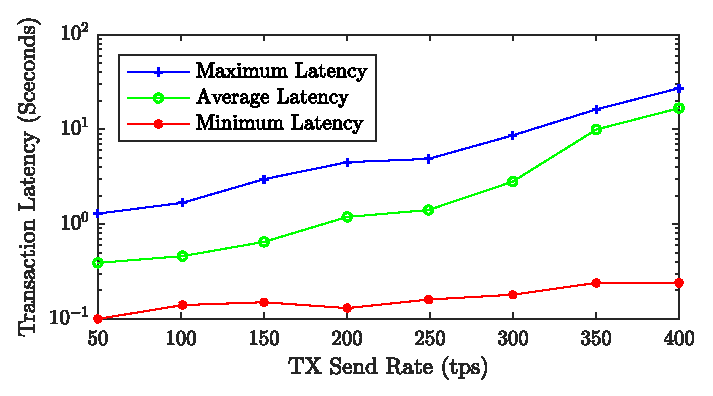
\includegraphics[width=\columnwidth]{Figures/ICBC-latency.eps}%
\caption{Send Rate V. Latency}%
\label{fig_latency_bc_pon}%
\end{subfigure}\hfill%
\begin{subfigure}{0.7\columnwidth}
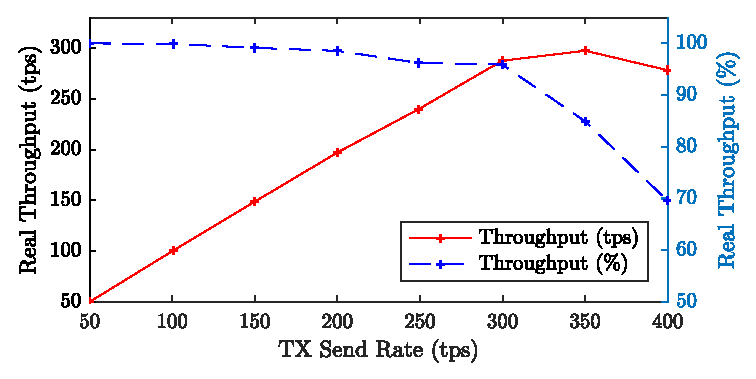
\includegraphics[width=\columnwidth]{Figures/ICBC-tps.eps}%
\caption{Send Rate V. Transaction Throughput}
\label{fig_TPS_bc_pon}
\end{subfigure}\hfill%
%\vspace{-4mm}
\caption{Benchmark Results: Send Rate V. Latency and Transaction Throughput}
\label{fig_results_bc_pon}%
%\vspace{-5mm}
\end{figure*}
% \textcolor{red}{Without more explanation the results don't say much to me. For OFC the CPU/memory/network usage might not be of interest. 
% The transaction latency could be but you first have to say why it is important that latency is low and relate it to some other performance. e.g., if latency is above a certain value, then you loose a certain efficiency. In short you use the first part of the paper to say what the issue is first in general and then specifically to the use case you consider. The second part described ion detail the issue with the use case and how it is modelled. The third part describes the experiment and results, and the result should relate back to the issue . you mentioned before and show how you improve the state of the art to solve that issue.}

% %\vspace{-4mm}

% \textcolor{red}{In Fig. 4.b, the Throughput \% should have its own y axis on the right hand side. This way you can also spread it better across the full size of the figure}

We run the experiments for 20,000 auction transactions with gradually increasing send rates from 50 to 400 \ac{TPS}. \figureautorefname~\ref{fig_results_bc_pon} illustrates the benchmark results of the auction application deployed on the Hyperledger Fabric network. The maximum, average, and minimum transaction latency under different send rates are shown in \figureautorefname~\ref{fig_latency_bc_pon}. As the transactions are sent to the network with a higher rate, the latency increases considerably. The system under test has been set up with adequate resources in order to minimize the computing power dependency of the results. Thus the radical increase in average latency for scenarios with more than 300 transactions per second means we are reaching the current scalability performance of the Hyperledger Fabric framework. %This is also confirmed by the big drop in transaction throughput in \figureautorefname~\ref{fig_TPS_bc_pon} when going beyond 300 \ac{TPS} where the throughput drops from 95\% to 84\% and then to 69\% when the send rate reaches 400 \ac{TPS}.

% It should be noted that for our application, the latency is not a limiting factor since the blockchain is used to verify the auctions after they have occurred, to disincentive any market manipulation by the \ac{InP}. The number of transactions per second is instead important to determine the aggregation factor of each auction. 

% \subsection{Conclusions}
In this section, we proposed a distributed market mechanism for \ac{PON} sharing where reliance on a central intermediary is mitigated and replaced by a blockchain-based smart contract. The smart contract assures reliable conduct of the market by holding the \acp{VNO} accountable through verifying the outcome of the auction mechanism using an endorsement policy.
In conclusion, our current result of achieving 300 transactions per second, before the performance drop (shown in \figureautorefname~\ref{fig_TPS_bc_pon}), provides the ability to verify upstream capacity blocks, each aggregating 25 upstream frames (i.e., every ~3 milliseconds), demonstrating the ability to prevent and promptly detect market manipulations.
In parallel, improving the throughput capacity of Hyperledger Fabric is also being pursued by researchers \cite{Gorenflo_2019}. In the future, we plan to make use of the smart contract technology to enhance the mechanism introduced in this section with automatically enforceable quality assurance and \ac{SLA} management.





\section{Distributed \ac{5G} Network Slicing Marketplace}
\label{BC:sec:slicing}

% \subsection{Introduction}
% \label{sec:intro}

What differentiates 5G from its predecessor generations of cellular communications is that it goes beyond merely multiplying the network capacity and speed and promises an ambitious vision where various services with vastly different functional requirements are seamlessly hosted over the same physical infrastructure without affecting each others' performance \cite{7980666}. This vision, in addition to many technical and standardization challenges that need to be addressed, demands a new approach to business and ownership models of network infrastructure \cite{Nima-5g-evol}, where automated resource orchestration and provisioning mechanisms handle on-demand resource needs of the operators. 
The most prominent model of resource allocation for 5G networks is slicing, which allows building customized logical networks on top of a shared physical infrastructure \cite{FCC_slicing}. Thanks to the virtualization technologies, it is now possible to allocate virtual instances of the physical infrastructure while assuring seamless functionality using slice isolation techniques.
As envisioned by \ac{3GPP} \cite{3gpp_tr_2018} in a highly heterogeneous network sharing ecosystem, network slices could be created to accommodate different functional and performance requirements of the network operators. This vision could see the emergence of a new market where a wide range of network operators, infrastructure providers, or public authorities carry out highly frequent transactions involving the exchange of resources, financial commitments, and post-deal operations. In other words, the conventional manual processing of these transactions is not feasible; therefore, novel automated process management methods have to replace them.
The new automated process management has to enable flexible resource provisioning for key players of this market and accommodate their quantitative and qualitative expectations from the network resources dedicated to them.


Typical business processes in the communications industry include economic models (e.g., auctions) that aim to solve resource management problems using pricing and allocation mechanisms \cite{8480631}. The main objective of these mechanisms, including the slice brokering \cite{8542782} is to efficiently allocate the available resources to the parties with the most critical demand while assuring the manipulation-proofness of the scheme. Nonetheless, the common assumption in these studies is the existence of an impartial central authority who could be trusted to conduct the market operations and execute the business processes without manipulating the outcome to its or another party's benefit. We will challenge this assumption throughout this section and will illustrate how blockchain technology, along with smart contracts, could provide a distributed alternative to the conventional centralized approach to slice brokering. Blockchain technology has already proven to provide solutions for similar problems in various trust-less industrial ecosystems such as healthcare \cite{mettler2016blockchain}, manufacturing \cite{abeyratne2016blockchain}, and banking \cite{guo2016blockchain}.

To the best of our knowledge, this section presents the first pragmatic implementation of a blockchain application for network slice brokering where the blockchain network is distributed on a commercial cloud environment and depicts realistic network/system-level \acp{KPI} such as latency, throughput, and computing resources. These realistic performance indicators are critical for providing a practical feasibility analysis of the proposed distributed slice brokering market.


Network slicing provides a solution to the diverse infrastructure/resource requirements of modern telecommunication networks. This is done through generating on-demand virtual instances of an end-to-end network on a physical infrastructure \cite{santos2018orchestration}. This enables service providers to serve their end-users with the utmost flexibility. 

In \cite{7514161}, the authors have reviewed the business requirements and standards in the context of multi-tenant mobile networks. They have introduced in detail the architecture of the 5G network slice broker. The idea of the on-demand capacity broker is to enable allocating a portion of the network capacity for a specific time slot to a secondary resource user (\ac{MVNO} or \ac{OTT} provider). They define a network slice as follow:
\begin{quote}
    "A network slice refers to an isolated amount of network capacity customized to best suit specific service requirements \cite{7514161}."
\end{quote}
In other words, a network slice is considered a complex commodity comprised of various resources required for providing services over a network. This commodity (network slice) is traded in a market in the form of leasing (temporary ownership) for a particular time-slot with pre-negotiated quantitative measures. The key factors in defining a network slice are:
\begin{itemize}
    \item The composition of the slice (quantitative description of the slice components, e.g., \ac{RAN}, computing, and storage)
    \item The time duration of the leasing.
    \item The metrics that determine the expected performance of the slice (e.g., availability, \ac{QoS} usually in the form of a \ac{SLA}).
\end{itemize}

% In the rest of this section, we will elaborate on the definition of a network slice as a commodity and provide a short review of its common market mechanisms. Furthermore, we discuss the need for quality assurance and the tools for enforcing the terms of the trade. 

Considering the above definition, a network slice can be treated as a commodity with a typical supply-chain which has to be sourced from multiple suppliers (the \acp{InP} or other \acp{MVNO} who are willing to share parts of their idle resources) and be delivered to an intermediary business customer who then would serve its end-users using this network slice.
Therefore the first function of the network slicing supply chain is the sourcing of the slice, i.e., acquiring the required resources for creating a slice with a particular configuration. From the slice requester's perspective, the aim is to acquire the slice with the necessary configuration for the lowest price from the market. On the other hand, from the suppliers' (the \ac{InP} or \acp{MVNO} with excess resources) point of view, the optimal outcome is for the slice to be sold for the highest possible price. Game theory has been widely used for similar markets in communications research where multiple players are involved on both sides of the market \cite{CHARILAS20103421}. 
Auctions, in particular, are very popular as market resolution tools \cite{8480631}. The resources that are traded in these resource markets range from spatial streams \cite{7842378} to spectrum/antennas \cite{7600959}, and resource blocks \cite{resource_blocks_auction}.
\begin{figure}[htbp]
            % \vspace{-4mm}
    \centering
    \includegraphics[width=0.8\columnwidth]{Figures/ICC-model.pdf}
    \caption{The Slice Broker Model}
    \label{fig:Slice_broker}
            % \vspace{-2mm}
\end{figure}
% \tochange{This is written like the prev work sec of a paper. I would reduce the refs but say more on why are they so relevant, maybe write it more as a story rather than a list of references}


Among these game-theoretical solutions, we are more specifically interested in auction mechanisms that are capable of handling multiple traders in both the selling and buying sides of the market. Such two-sided auctions are referred to as double auctions in the literature. A slice broker equipped with a double auction would allow service providers, network operators and infrastructure owners to participate in a market capable of creating on-demand network slices (depicted in \autoref{fig:Slice_broker}). A vertical market for network slices will provide new network infrastructure monetization opportunities by welcoming new market players (e.g., automotive industry,
e-health, etc.) and increasing the infrastructure utilization
through multiplexing gains provided by more slice requests \cite{ONETS}. Double auctions will further enhance the slice brokering operation by allowing the operators to monetize their underutilized resources. 


% In \cite{7794896}, the authors have proposed a flow-level slice brokering using an iterative double auction with a transaction cost. In their \ac{SDN}-based architecture, the \ac{SDN} controller acts as a broker and arranges the double-sided auction. Using simulations, they demonstrate the effectiveness and eventual convergence of their proposed iterative auction algorithm.
% A truthful double auction mechanism for spectrum slicing in virtualized wireless networks is proposed in \cite{ei2017game}, where multiple base stations hold an amount of spectrum resources and multiple \acp{ISP} compete to lease them. The efficiency of their proposed system is evaluated in terms of utilities of the market players and the auctioneer's profit. 
% In \cite{8542782}, a double auction algorithm is proposed to address the problems of service function chain routing and \ac{NFV} price adjustment. The \ac{NFV} broker acts as the central auctioneer who received the bids and ask prices from the customers/suppliers and decides on the allocation and pricing of the resources. 

% \textbf{In the previous section}, we described the \ac{5G} slice brokering and defined the structure of the market.
% The slice brokering mechanisms have 

Multiple placement options for the slice broker have been proposed in the literature (e.g., in the SDN controller \cite{7794896} or the orchestrator \cite{7514161}). However, what is common with most of these proposals is that the brokering mechanism is hosted by a single entity that is not necessarily impartial and might have incentives to manipulate the outcomes of the mechanism. In this section, we propose a distributed slice brokering model which allows two-sided trade of the resources required to create a slice of the network. The traded commodity in this market is either a unit-bundle of different resource types (\ac{RAN}, computing, or storage) or a single type multiple-unit of each resource type. The distributed brokering model is based on smart contract technology and mitigates the reliance on a central authority to operate the slice broker.

The application of blockchain technology for slice brokering have been previously studied in the literature.
In \cite{8368983}, the authors present a feasibility analysis of a network slice broker using blockchain that enables dynamic slice acquisition for automated industrial processes. Their results show that the analyzed industrial micro-processes can benefit from adopting a blockchain-based \ac{5G} network slice broker and the distributed ledger technology. However, the authors have not endeavored to implement the use case on the blockchain and have settled for theoretical analysis. The authors in \cite{8707070} have proposed a blockchain-based network slice broker for 5G services to secure and ensure anonymous transactions using blockchain. They have developed a proof of concept to evaluate the performance of their proposed slice broker. Their proposed blockchain platform is based on a consensus mechanism called Hashcash \cite{hashcash}. Their performance evaluation is, however, only limited to comparing the average time of sub-slice contract creation and slice deployment. They conclude that the additional security and privacy provided by blockchain does not have a significant impact on the performance of the slice broker. Hashcash is a public blockchain that uses a \ac{PoW} based consensus protocol which relies on the network nodes solving computationally complex problems to reach consensus \cite{8716424}. Although \ac{PoW} consensus due to its pseudo-anonymous nature could be the most robust and secure option for particular applications (e.g., crypto-currencies), in enterprise ecosystems such as telecoms, they appear to be redundant as the parties involved in the blockchain are already known to each other. Therefore, permissioned blockchains that are designed for enterprise ecosystems and use more straightforward and less resource consuming consensus protocols such as Raft \cite{Ongaro:raft} are considered a better fit.


% \towrite{Maybe add a figure with slice combinations}

In this section, we use an implementation of the double auction mechanism introduced in \autoref{cpt:chapter_2}, which enables multiple traders in both sides (seller/buyer) of the market to trade their resources (multiple items simultaneously). The double auction mechanism assures manipulation-proofness of the market by decoupling the ask/bid value proposed by the traders from the final price paid; therefore, the traders cannot manipulate the market by strategizing over their proposed ask/bid value. %The steps of the auction transaction are further explained in section \ref{sec:results}.
We deploy the slice broker application on a realistic distributed implementation of Hyperledger Fabric to be able to evaluate the performance of the market with the reflection of real-world network latency and processing. 

% Finally, in \cite{8808114} a blockchain-based architecture is proposed to secure customized network slices. They make use of the concept of multiple channels in Hyperledger Fabric and provide isolation and privacy-preservation to orchestration operations of network slices. 
% The focus of this work is however \textcolor{red}{on ....}, rather than slice brokering. 





\begin{figure}%[htbp]
    \centering
    \includegraphics[width=0.8\columnwidth]{Figures/txFlow.pdf}
    \caption{The Distributed Broker Transaction Flow}
    \label{fig:txFlow}
\end{figure}
\towrite{You don't really describe the usecase it's difficult to say how this can relate to a specific 5G usecase.}
\towrite{The way it's described it can be applied to anything maybe you need}
The transaction flow in our proposed distributed slice brokering is depicted in \autoref{fig:txFlow}. First, the transaction proposals are sent to the blockchain peers. A transaction proposal consists of a table of ask/bid values, and the quantity of available/demanded resources proposed by each \ac{VNO} along with the proposed (unverified) outcome of the double auction, which determines the identity of the winning traders and the quantity of trades. This process is initiated inside the client application and then broadcast to the peers of each blockchain member \ac{VNO}. Once the peers receive the transactions, they begin the endorsement process by executing the chaincode, which contains an implementation of the brokering auction mechanism. If the resource allocation outcome resulting from the peer-run auction matches the proposed outcome, they endorse the transaction by returning a signed transaction. When enough number of endorsements is reached (this number depends on the endorsement policy that in our case is N-out-of-N, i.e., all the peers have to endorse), the transactions are sent to the ordering service, where the consensus is reached (i.e., Raft in our case). The final block is then created and committed to the ledger. Therefore, this distributed process replaces the conventional centralized approach to slice brokering, where a single authority does not control the entire conduct of the market.
\subsection{System Implementation and Results}
\label{sec:results}

\begin{figure*}%[htbp]
% \vspace{-2mm}
    \centering
    \includegraphics[width=0.99\textwidth]{Figures/ICC-vms1.pdf}
    \caption{The Experimental Setup: Blockchain Network Architecture}
    \label{fig:Arcitecture}
                % \vspace{-5mm}
\end{figure*}
We use the Hyperledger Fabric (version 1.4.1) framework to implement our blockchain application. To achieve realistic results, we deploy an under-laying network of nodes similar to a real-world production environment. The \ac{SUT} shown in \figureautorefname~\ref{fig:Arcitecture} consists of 6 \ac{VM} instances. \ac{VM}1 (8 \acp{vCPU} Intel(R) Xeon(R) @ 2.30GHz and 32 GB memory) hosts Hyperledger Caliper \cite{caliper} which is a benchmark tool designed to measure the performance of multiple blockchain solutions. The blockchain network consists of 5 organizations, each hosting one instance of a peer, orderer, chaincode, and certificate authority (see \autoref{Back:Sec:blockchain}). These blockchain components are each deployed as a Docker container, and Docker Swarm is used to orchestrate the containers that are distributed across a network of \acp{VM}. \ac{VM}1 is the Docker Swarm manager which is in charge of composing and deploying the containers at the beginning of the benchmark. \ac{VM}2-\ac{VM}6 (4 \acp{vCPU} and 15 GB memory) each host an organization and their containers. This provides a realistic implementation, where different organizations run their processing in different and independent virtual machines. %The benchmark begins with the Hyperledger Caliper generating the transaction proposals and sending them to the peers at a fixed-rate. The transaction information consists of a table of ask/bid values proposed by each trader along with the proposed (unverified) outcome of the double auction allocation of the resources. This process is initiated inside the client application and then broadcast to the peers of each blockchain organization. Once the peers receive the transactions, they begin the endorsement process by executing the chaincode, which contains an implementation of the auction mechanism. If the resource allocation outcome resulting from the peer-run auction matches the proposed outcome, they endorse the transaction by returning a signed transaction. When enough number of endorsements are reached (this number depends on the endorsement policy that in our case is N-out-of-N i.e., all the peers have to endorse), the transactions are sent to the Ordering Service, where the consensus is reached (i.e., Raft in our case). The final block is then created and committed to the ledger.



The experiment consists of multiple rounds of benchmarks with varying transaction send rates (from 20 to 110 \ac{TPS}). For each benchmark, we generate 10,000 transactions (i.e., each transaction is one round of double auction) and submit them to the blockchain to measure the minimum, average and maximum transaction latency and transaction throughput. In addition, to evaluate the container-level computing and network resource utilization of the blockchain application, we use Prometheus \cite{prometheus}, an open-source monitoring system, to record real-time metrics in a time-series database and then visualize these metrics using Grafana \cite{grafana} visualization suite.


\begin{figure*}[htbp]
% \vspace{-2mm}
\centering
\begin{subfigure}{0.7\columnwidth}
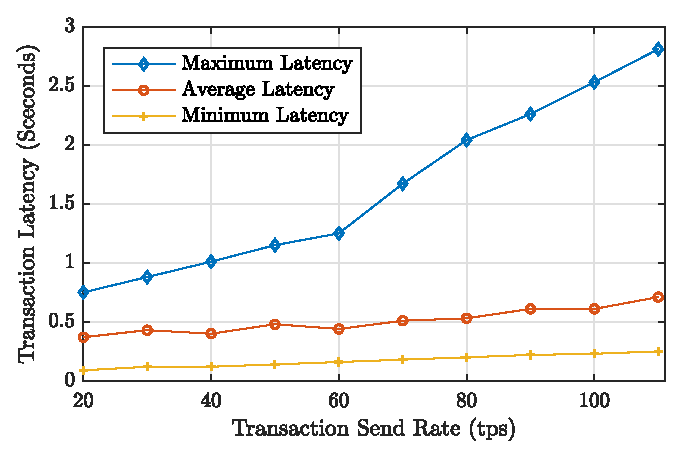
\includegraphics[width=\columnwidth]{Figures/ICC-latency.eps}%
\caption{Send Rate V. Latency}%
\label{fig_latency}%
\end{subfigure}\hfill%
\begin{subfigure}{0.7\columnwidth}
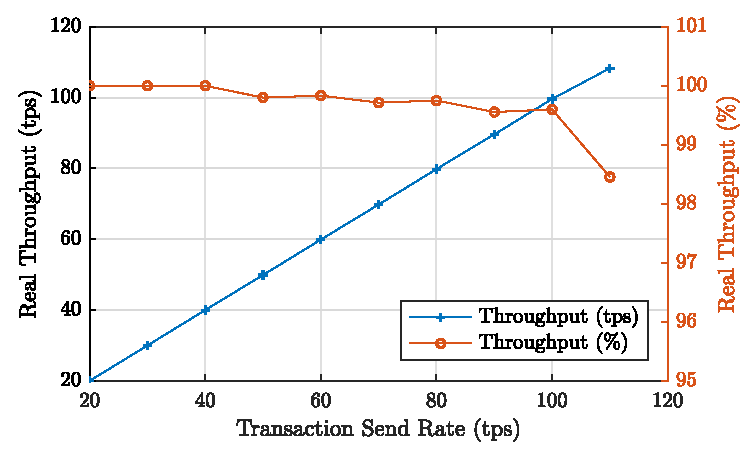
\includegraphics[width=\columnwidth]{Figures/ICC-tps.eps}%
\caption{Send Rate V. Transaction Throughput}
\label{fig_TPS}
\end{subfigure}\hfill%
% \vspace{-4mm}
\caption{Benchmark Results: Send Rate V. Latency and Transaction Throughput}
\label{fig_results}%
% \vspace{-5mm}
\end{figure*}

\tochange{is the algorithm/smart contract difeerent than the prev usecase?\autoref{fig_results}}

\tochange{What hapens if increase TPS further beyond 110? \autoref{fig_TPS}}



The minimum, average, and maximum transaction latency for each experiment is shown in \figureautorefname~\ref{fig_latency}. The minimum and average latency follow a semi-linear growth (with a different slope) as the send rate increases. The average latency remains below 1 second throughout the experiments. The maximum latency, on the other hand, grows more rapidly compared to the minimum and average latency and goes beyond 1 second as the send rate reaches 50 \ac{TPS}. In real-time applications, the maximum latency is the bounding metric as it determines the feasibility of the application. The maximum latency, however, can be controlled using transaction processing timeouts, where necessary, and a default output for the transaction is defined. \figureautorefname~\ref{fig_TPS} illustrates the transaction throughput of the blockchain application based on varying send rate. The throughput remains above 99.5\% while the send rate is up to 100 \ac{TPS}. However, a significant drop (down to 98.4\%) in the throughput is experienced as the send rate is raised to 110 \ac{TPS}, showing we have reached the highest usable rate.


\begin{figure}%[htbp]
% \vspace{-4mm}
\centering
\begin{subfigure}{0.7\columnwidth}
\includegraphics[width=\columnwidth]{Figures/ICC-cpu.pdf}%
\caption{\ac{CPU} Utilization}%
\label{fig:cpu}%
\end{subfigure}\hfill%
\begin{subfigure}{0.7\columnwidth}
\includegraphics[width=\columnwidth]{Figures/ICC-mem.pdf}%
\caption{Memory Utilization}
\label{fig:mem}
\end{subfigure}\hfill%
\begin{subfigure}{0.7\columnwidth}
\includegraphics[width=\columnwidth]{Figures/ICC-net.pdf}%
\caption{Network Utilization}
\label{fig:net}
\end{subfigure}\hfill%
\caption{Benchmark Results: Send Rate V. Latency, Throughput}
\label{fig_results2}%
% \vspace{-8mm}
\end{figure}
% \begin{figure}[tb]\ContinuedFloat
% % \vspace{-4mm}
% \begin{subfigure}{0.7\columnwidth}
% \includegraphics[width=\columnwidth]{Figures/ICC-net.pdf}%
% \caption{Network Utilization}
% \label{fig:net}
% \end{subfigure}\hfill%
% % \vspace{-4mm}
% % \caption{Benchmark Results: Send Rate V. Latency and Transaction Throughput}
% % \label{fig_results2}%
% % \vspace{-8mm}
% \end{figure}


Throughout each experiment, 20 docker containers are created and deployed on top of an overlay network to which all the \acp{VM} are connected. To get a better insight into the resource consumption and, therefore, the infrastructure footprint of the blockchain application, we have produced \figureautorefname~\ref{fig_results2}, which depicts the container-specific \ac{CPU}, memory and network utilization throughout one instance of the experiment. %(100 tps * 10,000)
As previously mentioned, each component of the blockchain is implemented as a Docker container. For the purpose of clarity, \ac{CA} containers are intentionally omitted from the visualization as their resource consumption is negligible. 
\figureautorefname~\ref{fig:cpu} depicts the \ac{CPU} utilization of the containers. The peer nodes (tasked with the endorsement of the transactions) are using most \ac{CPU} resources. This is due to the fact that the verification of the smart contracts (auction) outcome is done by the peers; hence, the high \ac{CPU} usage. 
The memory consumption is illustrated in \figureautorefname~\ref{fig:mem}, where the peer nodes are consuming the most memory, followed by the orderers that also consume a considerable amount.
\figureautorefname~\ref{fig:net} shows the sum of incoming and outgoing network traffic to/from each container. As expected, the orderers occupy the biggest part of the network due to the highly-frequent signaling among the orderers to reach consensus. 
\towrite{Any usefull conclution or guidline you can make from these figures?}

In this section, we proposed a distributed market design for \ac{5G} network slicing based on blockchain technology. We implemented a variant of the double auction mechanism as a smart contract to assure trust in a telcoms business ecosystem, where no trusted authority could control the resource sharing market mechanism. We have deployed a pragmatic network of blockchain nodes over six cloud-hosted \acp{VM} to achieve realistic performance measurements. Using the deployed blockchain application, which is powered by the Hyperledger Fabric framework, we conducted an analysis of the blockchain network performance in terms of latency and transaction throughput. These metrics are essential in designing blockchain-based markets as they determine the feasibility and frequency of resource trades over blockchain. Our experiments showed that our blockchain slicing market application is able to process up to 40 auction transactions per second while maintaining a 100\% transaction throughput and an average latency of 500 milliseconds, with a maximum of 100 TPS, with throughout very close to 100 \%.
Meanwhile, as mentioned in \cite{valcarenghireliable}, the time-scale envisioned for a \ac{5G} network slice provisioning and deployment is in the order of minutes. Therefore, our proposed market could support the simultaneous and real-time provisioning of multiple \ac{5G} slices without imposing any considerable latency to the process.
% Here is the reference for the order of minutes: Within the research community, the 5G-Transformer project 14 envisions three functional layers for providing verticals with slices: a Vertical Slicer as the logical entry point for verticals to support the creation of their respective transport slices in a short time-scale (in the order of minutes), Page 5 of \cite{valcarenghireliable}
% and also another reference here: https://ieeexplore.ieee.org/document/8696471   This demo will show how a novel software framework based on the 5GT architecture can deploy a mobile network slice in a few minutes.


% In this paper we  a practical implementation of a market mechanism to address the slicing problem in \ac{5G} networks. However, the proposed platform could be used for other smart contracts with different logic covering interference etc.
% \vfill
\section{Conclusions}
\label{bc:sec:Conclusions}
In this chapter, we proposed a distributed market model for inter-operator network sharing. The proposed market model addresses the lack of trust in a central authority to conduct the market, which poses a threat to the adoption of markets in emerging network ownership models.
We introduced a distributed approach to the bilateral trade markets for future telecommunications networks. We first described the research areas where bilateral trade markets are being adopted and the game-theoretic solutions for the allocation of commodities. Then we argued that the current trust on the central third-party brokers might not be sustainable as new network ownership models will provide market manipulation incentives for these brokers. As the main contribution of this section, we illustrated how blockchain technology, along with smart contracts, can help the bilateral trade markets to function in an untrusted environment.

The proposed distributed market model provided an answer to the following research question: 

\textit{\RQe}

We picked two use cases from the telecommunications industry, where centralized decision making poses a limitation. The first use case (\autoref{BC:sec:pon}) is multi-tenant \ac{PON} excess capacity sharing market described in \autoref{cpt:chapter_2}. We proposed a verification layer enabled by the proposed smart contract to conduct the auctions in parallel with the \ac{InP} and therefore allow for auditing of the auction outcome as demanded by any of the parties. This is possible as the record of the market transaction is kept in the distributed ledger on the blockchain network.

The second use case is network slicing in \ac{5G} where the network operators, \acp{InP}, and \acp{OTT} could source the resources (\ac{RAN}, computing, storage, etc.) required for their network slice from other parties using the provided market mechanism. The novelty of this use case is eliminating the dependency on a central broker to conduct the market and match the sellers and buyers. 

To examine the feasibility of our proposals, we implemented the proposed market models using an open-source blockchain framework, Hyperledger Fabric. Finally, we reported the results of our experiments and analyzed how the proposed distributed markets perform under different loads and also how these differences affect performance metrics such as latency and transaction throughput.
However, the performance of a blockchain system highly relies on the \ac{SUT} and other properties of the blockchain such as block size, authorization methods, and consensus protocol. Therefore, further research is needed to asses the effect of these design choices on the \ac{5G} slicing market performance.


% addressing emerging network ownership models in telecommunications networks use cases. The proposed model is based on the smart contract technology and enables transparent and trusted bilateral trades, where trust among the network operators does not exist, and there is no impartial third-party entity who is trusted by all of the participants. We use an open source permissioned blockchain framework called Hyperledger Fabric to investigate the performance of the distributed market mechanism in cloud environments. After running experiments on Hyperledger Fabric, we discuss the practical feasibility and possible design choices of our blockchain approach based on latency, throughput and resource consumption analysis.


% \section{Dissemination}
% \subsection{Peer-Reviewed}

%  \begin{enumerate}
   
%     \item  \textbf{\underline{N. {Afraz}}} and M.~{Ruffini}, ``A Distributed Bilateral Resource Market Mechanism for Future Telecommunications Networks,'' in \emph{2019 IEEE Global Communications Conference (GLOBECOM)}, December 2019.

%     \item H.~Ahmadi, I.~Macaluso, M.~{Ruffini}, \textbf{\underline{N. {Afraz}}}, ``blockchain Technology and Smart Contracts in \ac{5G} and Beyond Networks [Tutorial Talk],'' 2019, European Conferences on Networks and Communications (EUCNC).
    
%     \item {A. {Khatoon}}, \textbf{\underline{N. {Afraz}}}, ``Approaches to Adopt Blockchain Technology for the Internet of Things,'' in IEEE Technology and Society Magazine, under review.


%  \end{enumerate}
%  \subsection{Non Peer-Reviewed}
%  \begin{enumerate}

%     \item \textbf{\underline{N. {Afraz}}}, V.~Chaudhary \emph{et~al.}, ``Optimizing Wholesale Intercarrier Settlement with Hyperledger Fabric blockchain,'' in \emph{Solution Brief}.\hskip 1em plus 0.5em minus 0.4em\relax Telecom Special Interest Group, 2019.

%     % \item \bibentry{Nima-telecom-sig}
%     % \item \bibentry{Nima-osa}
%  \end{enumerate}